% Options for packages loaded elsewhere
\PassOptionsToPackage{unicode}{hyperref}
\PassOptionsToPackage{hyphens}{url}
%
\documentclass[
]{article}
\usepackage{amsmath,amssymb}
\usepackage{iftex}
\ifPDFTeX
  \usepackage[T1]{fontenc}
  \usepackage[utf8]{inputenc}
  \usepackage{textcomp} % provide euro and other symbols
\else % if luatex or xetex
  \usepackage{unicode-math} % this also loads fontspec
  \defaultfontfeatures{Scale=MatchLowercase}
  \defaultfontfeatures[\rmfamily]{Ligatures=TeX,Scale=1}
\fi
\usepackage{lmodern}
\ifPDFTeX\else
  % xetex/luatex font selection
\fi
% Use upquote if available, for straight quotes in verbatim environments
\IfFileExists{upquote.sty}{\usepackage{upquote}}{}
\IfFileExists{microtype.sty}{% use microtype if available
  \usepackage[]{microtype}
  \UseMicrotypeSet[protrusion]{basicmath} % disable protrusion for tt fonts
}{}
\makeatletter
\@ifundefined{KOMAClassName}{% if non-KOMA class
  \IfFileExists{parskip.sty}{%
    \usepackage{parskip}
  }{% else
    \setlength{\parindent}{0pt}
    \setlength{\parskip}{6pt plus 2pt minus 1pt}}
}{% if KOMA class
  \KOMAoptions{parskip=half}}
\makeatother
\usepackage{xcolor}
\usepackage[margin=1in]{geometry}
\usepackage{longtable,booktabs,array}
\usepackage{calc} % for calculating minipage widths
% Correct order of tables after \paragraph or \subparagraph
\usepackage{etoolbox}
\makeatletter
\patchcmd\longtable{\par}{\if@noskipsec\mbox{}\fi\par}{}{}
\makeatother
% Allow footnotes in longtable head/foot
\IfFileExists{footnotehyper.sty}{\usepackage{footnotehyper}}{\usepackage{footnote}}
\makesavenoteenv{longtable}
\usepackage{graphicx}
\makeatletter
\def\maxwidth{\ifdim\Gin@nat@width>\linewidth\linewidth\else\Gin@nat@width\fi}
\def\maxheight{\ifdim\Gin@nat@height>\textheight\textheight\else\Gin@nat@height\fi}
\makeatother
% Scale images if necessary, so that they will not overflow the page
% margins by default, and it is still possible to overwrite the defaults
% using explicit options in \includegraphics[width, height, ...]{}
\setkeys{Gin}{width=\maxwidth,height=\maxheight,keepaspectratio}
% Set default figure placement to htbp
\makeatletter
\def\fps@figure{htbp}
\makeatother
\setlength{\emergencystretch}{3em} % prevent overfull lines
\providecommand{\tightlist}{%
  \setlength{\itemsep}{0pt}\setlength{\parskip}{0pt}}
\setcounter{secnumdepth}{-\maxdimen} % remove section numbering
\ifLuaTeX
  \usepackage{selnolig}  % disable illegal ligatures
\fi
\usepackage{bookmark}
\IfFileExists{xurl.sty}{\usepackage{xurl}}{} % add URL line breaks if available
\urlstyle{same}
\hypersetup{
  pdftitle={FLIM Analysis Template},
  pdfauthor={Sevde Coban},
  hidelinks,
  pdfcreator={LaTeX via pandoc}}

\title{FLIM Analysis Template}
\author{Sevde Coban}
\date{2025-04-08}

\begin{document}
\maketitle

\section{Purpose}\label{purpose}

FLIM collects photon excitation information from cell images to examine
metabolic changes within biologic samples. This information is Fourier
transformed to collect two parameters: S-coordinate and G-coordinate.
These parameters are used to calculate fraction bound (fB), which is the
fraction of bound to unbound NADH within the cells we're looking at.
Fraction bound can tell you if the cells are using more glycolysis (more
free NADH) or oxidative phosphorylation (more NADH is bound to an
enzyme).

The purpose of this analysis is to compare the differences in fraction
bound (fB) between STA treated and untreated samples.

\section{Z' Factors for Fraction Bound and
G-Coordinates}\label{z-factors-for-fraction-bound-and-g-coordinates}

Here are the Z' factors for fB and G-Coordinate across the 3
experiments. Raw values are calculated using all individual measurements
for each sample. Mean values first average indiividual measurements
within each Sample\_ID then calculates Z' factors using the averaged
values. This minimizes intra-sample variability.

\begin{longtable}[]{@{}lr@{}}
\caption{Z' Factor per Run (fB)}\tabularnewline
\toprule\noalign{}
Experiment & z\_prime\_factor \\
\midrule\noalign{}
\endfirsthead
\toprule\noalign{}
Experiment & z\_prime\_factor \\
\midrule\noalign{}
\endhead
\bottomrule\noalign{}
\endlastfoot
EITM-USC\_run1 & -0.1959437 \\
EITM-USC\_run2 & -19.6521376 \\
EITM-USC\_run3 & 0.0248862 \\
\end{longtable}

\begin{longtable}[]{@{}lr@{}}
\caption{Z' Factor per Run (Average fB)}\tabularnewline
\toprule\noalign{}
Experiment & z\_prime\_factor \\
\midrule\noalign{}
\endfirsthead
\toprule\noalign{}
Experiment & z\_prime\_factor \\
\midrule\noalign{}
\endhead
\bottomrule\noalign{}
\endlastfoot
EITM-USC\_run1 & 0.5402899 \\
EITM-USC\_run2 & -2.2092288 \\
EITM-USC\_run3 & 0.8344722 \\
\end{longtable}

\begin{longtable}[]{@{}lr@{}}
\caption{Z' Factor per Run (G)}\tabularnewline
\toprule\noalign{}
Experiment & z\_prime\_factor \\
\midrule\noalign{}
\endfirsthead
\toprule\noalign{}
Experiment & z\_prime\_factor \\
\midrule\noalign{}
\endhead
\bottomrule\noalign{}
\endlastfoot
EITM-USC\_run1 & 0.1179575 \\
EITM-USC\_run2 & -19.7009225 \\
EITM-USC\_run3 & 0.1939339 \\
\end{longtable}

\begin{longtable}[]{@{}lr@{}}
\caption{Z' Factor per Run (Average G)}\tabularnewline
\toprule\noalign{}
Experiment & z\_prime\_factor \\
\midrule\noalign{}
\endfirsthead
\toprule\noalign{}
Experiment & z\_prime\_factor \\
\midrule\noalign{}
\endhead
\bottomrule\noalign{}
\endlastfoot
EITM-USC\_run1 & 0.6898841 \\
EITM-USC\_run2 & -4.4975397 \\
EITM-USC\_run3 & 0.8750364 \\
\end{longtable}

\section{Scatterplot of S- \& G- Coordinates of STA
Treatments}\label{scatterplot-of-s--g--coordinates-of-sta-treatments}

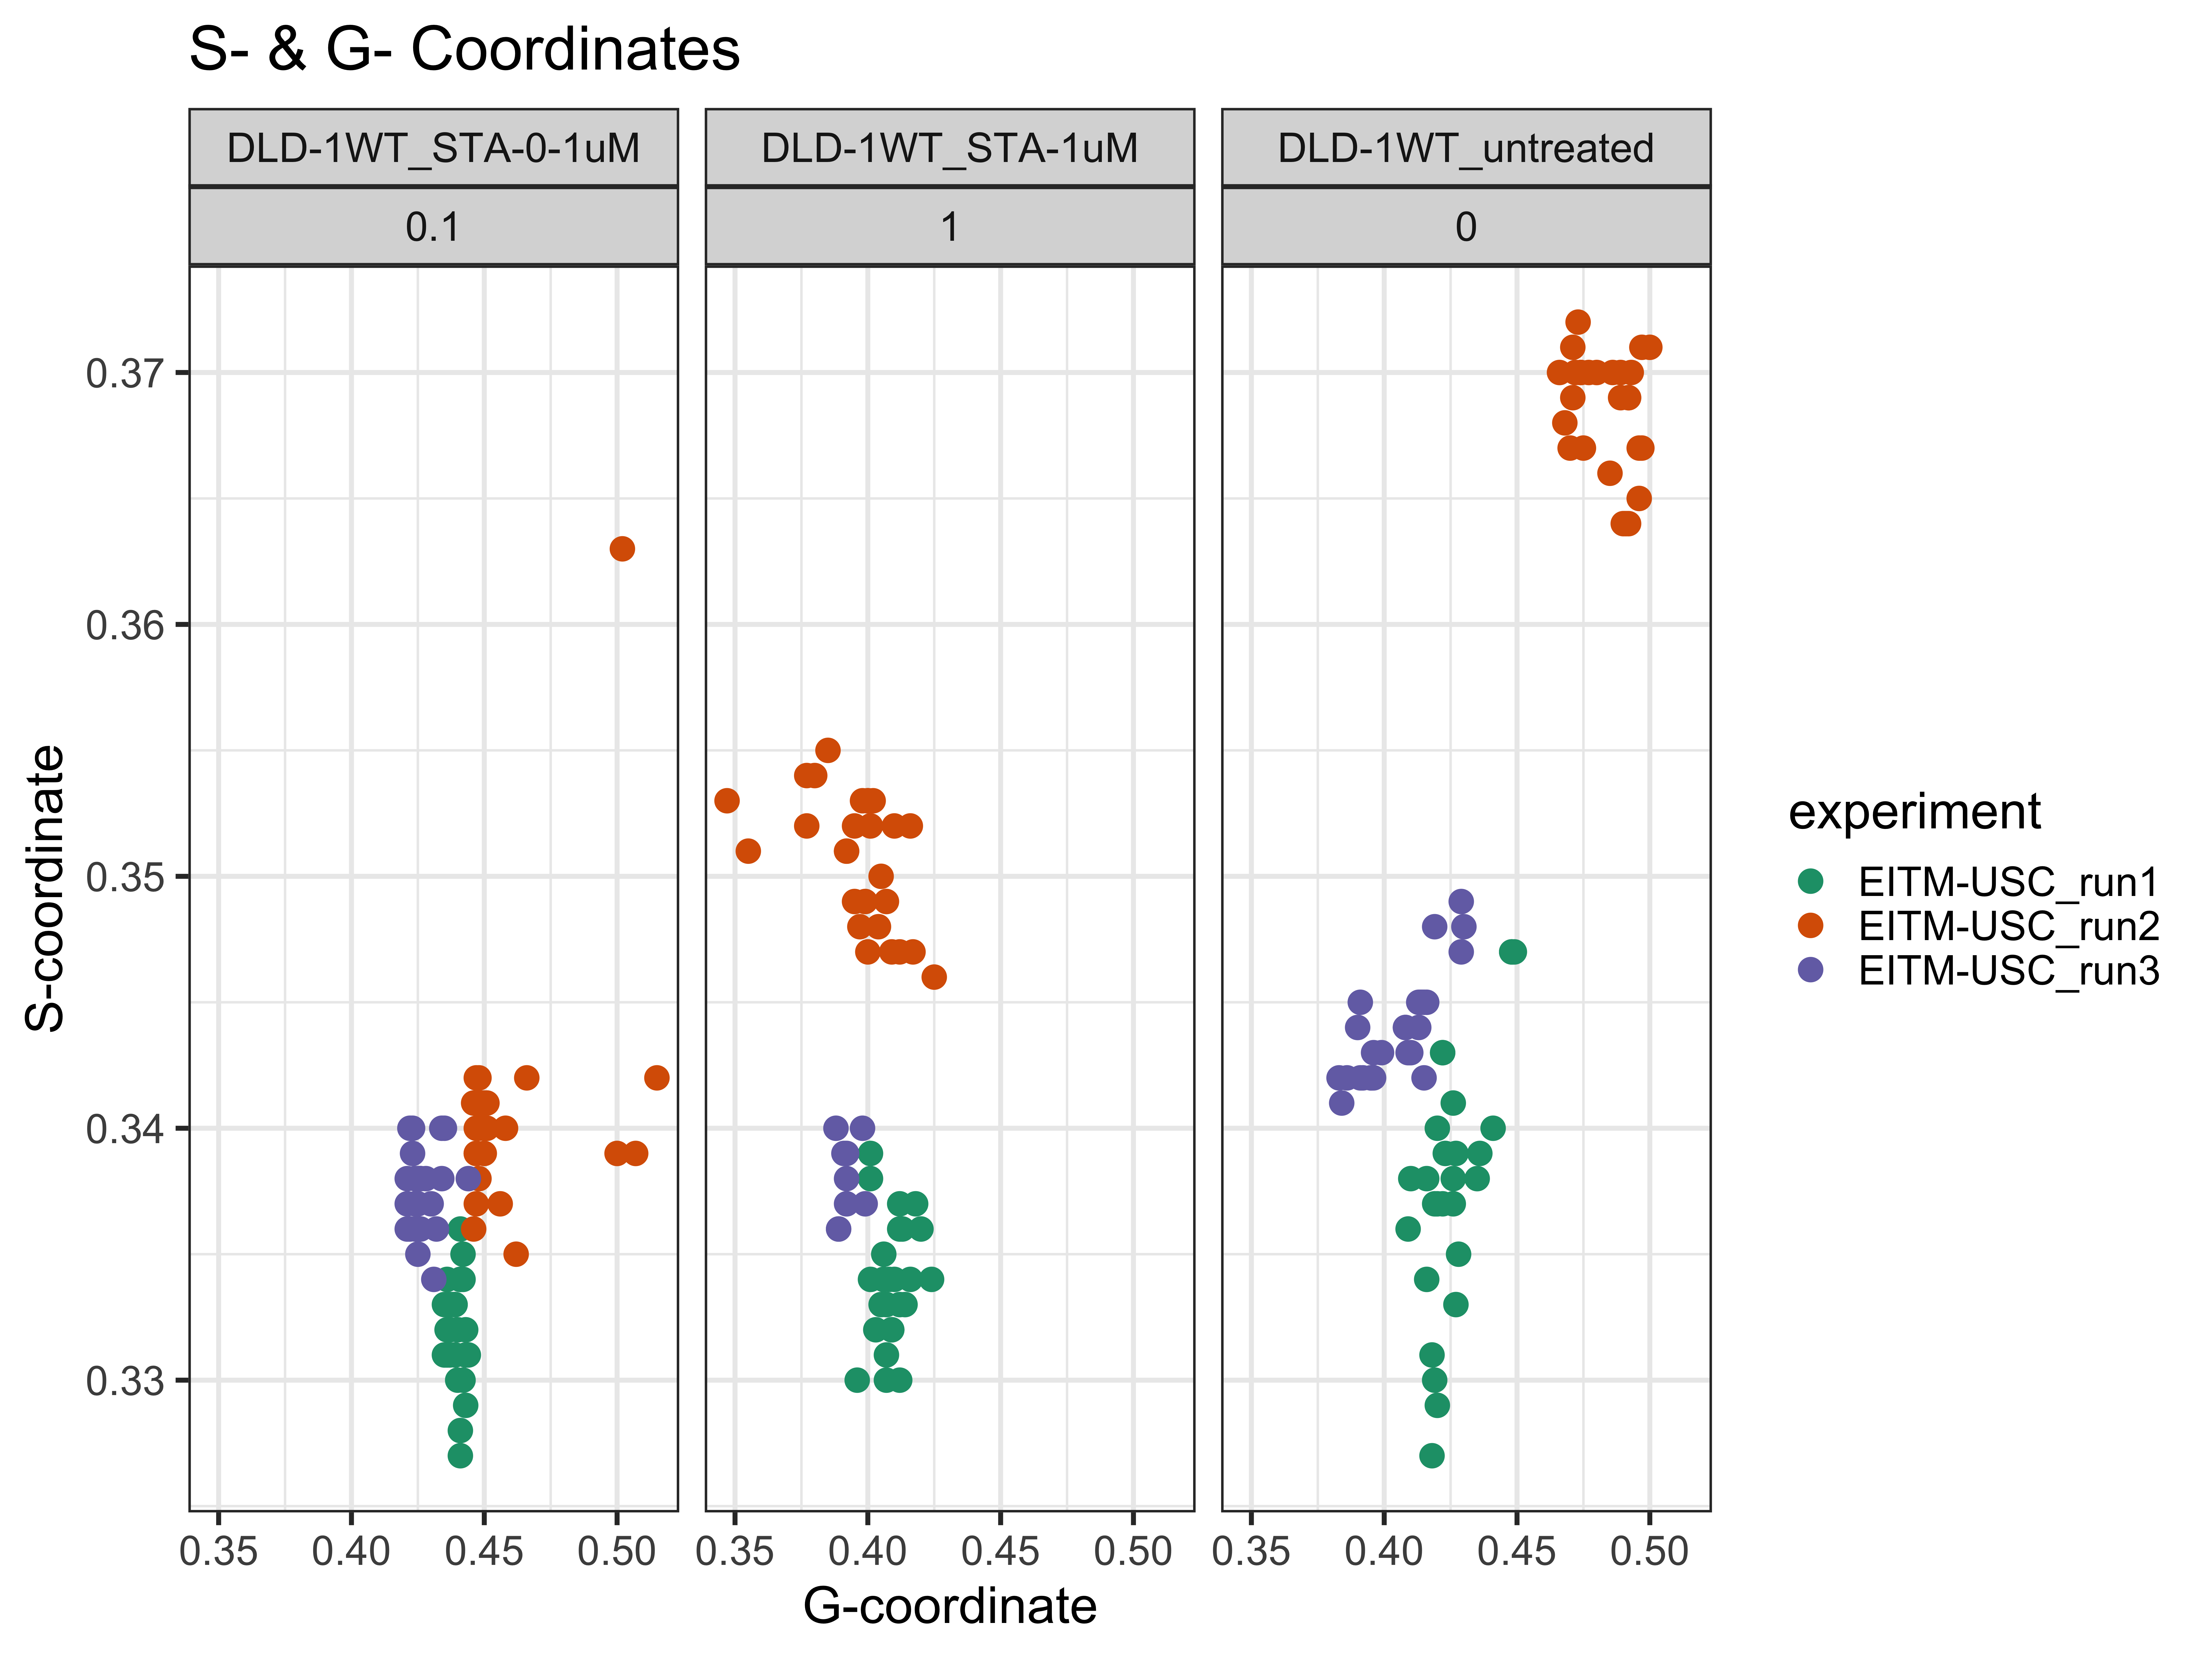
\includegraphics{FLIM_Analysis_Newdata_files/figure-latex/plot1-1.pdf}

\section{Mixed Effects Models (Fraction
Bound)}\label{mixed-effects-models-fraction-bound}

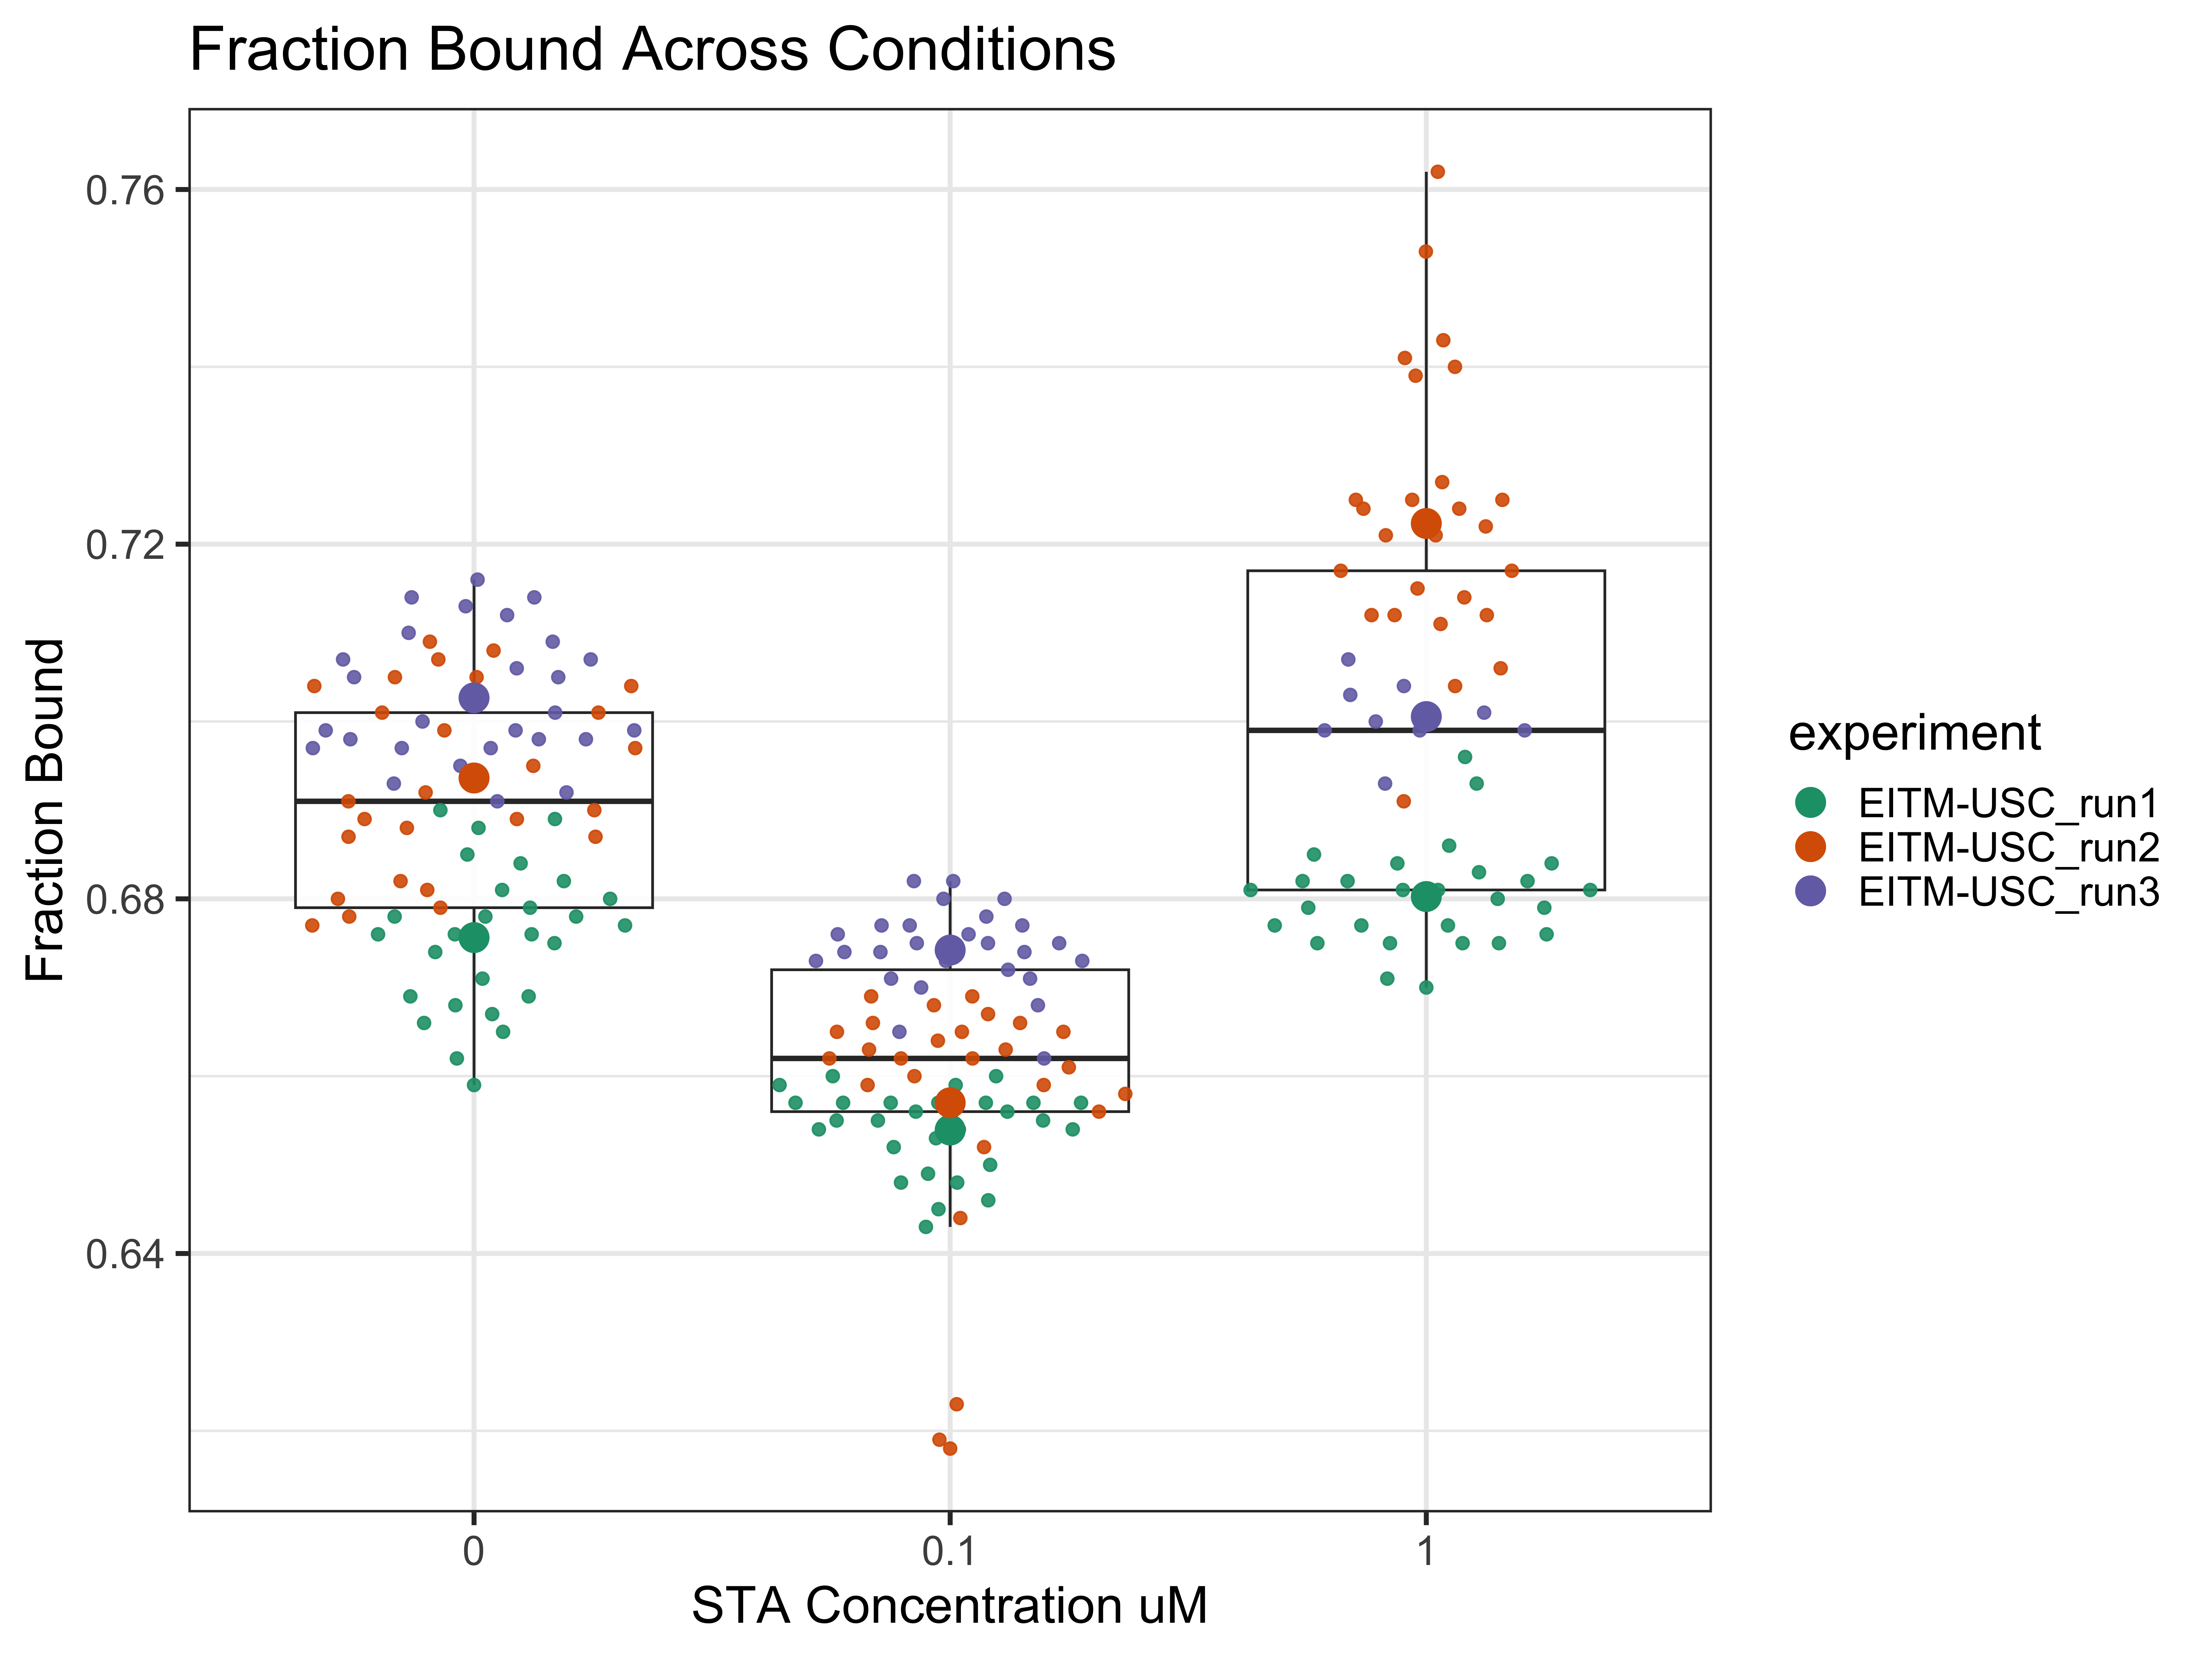
\includegraphics{FLIM_Analysis_Newdata_files/figure-latex/boxplot-1.pdf}
The goal of this experiment is to compare fraction bound (fB) across
varying concentrations of STA treatment. Each boxplot displays the
distribution of fB for a specific concentration, and each point is
color-coded by experimental run. You can see that the data tends to
cluster by run rather than purely by treatment. The data points from run
3 consistently appear higher across all conditions. This suggests that a
substantial percentage of the variation in fB is attributable to
differences between experiment runs, rather than just treatment effects.
This is not suprising because FLIM is a variable assay and there can be
fluctuations between runs resulting in variations in the data.

To account for this, we use a mixed-effects model, with STA
concentration as a fixed effects and experiment (run) as a random effect
in order to isolate the effect of STA treatment on fB.

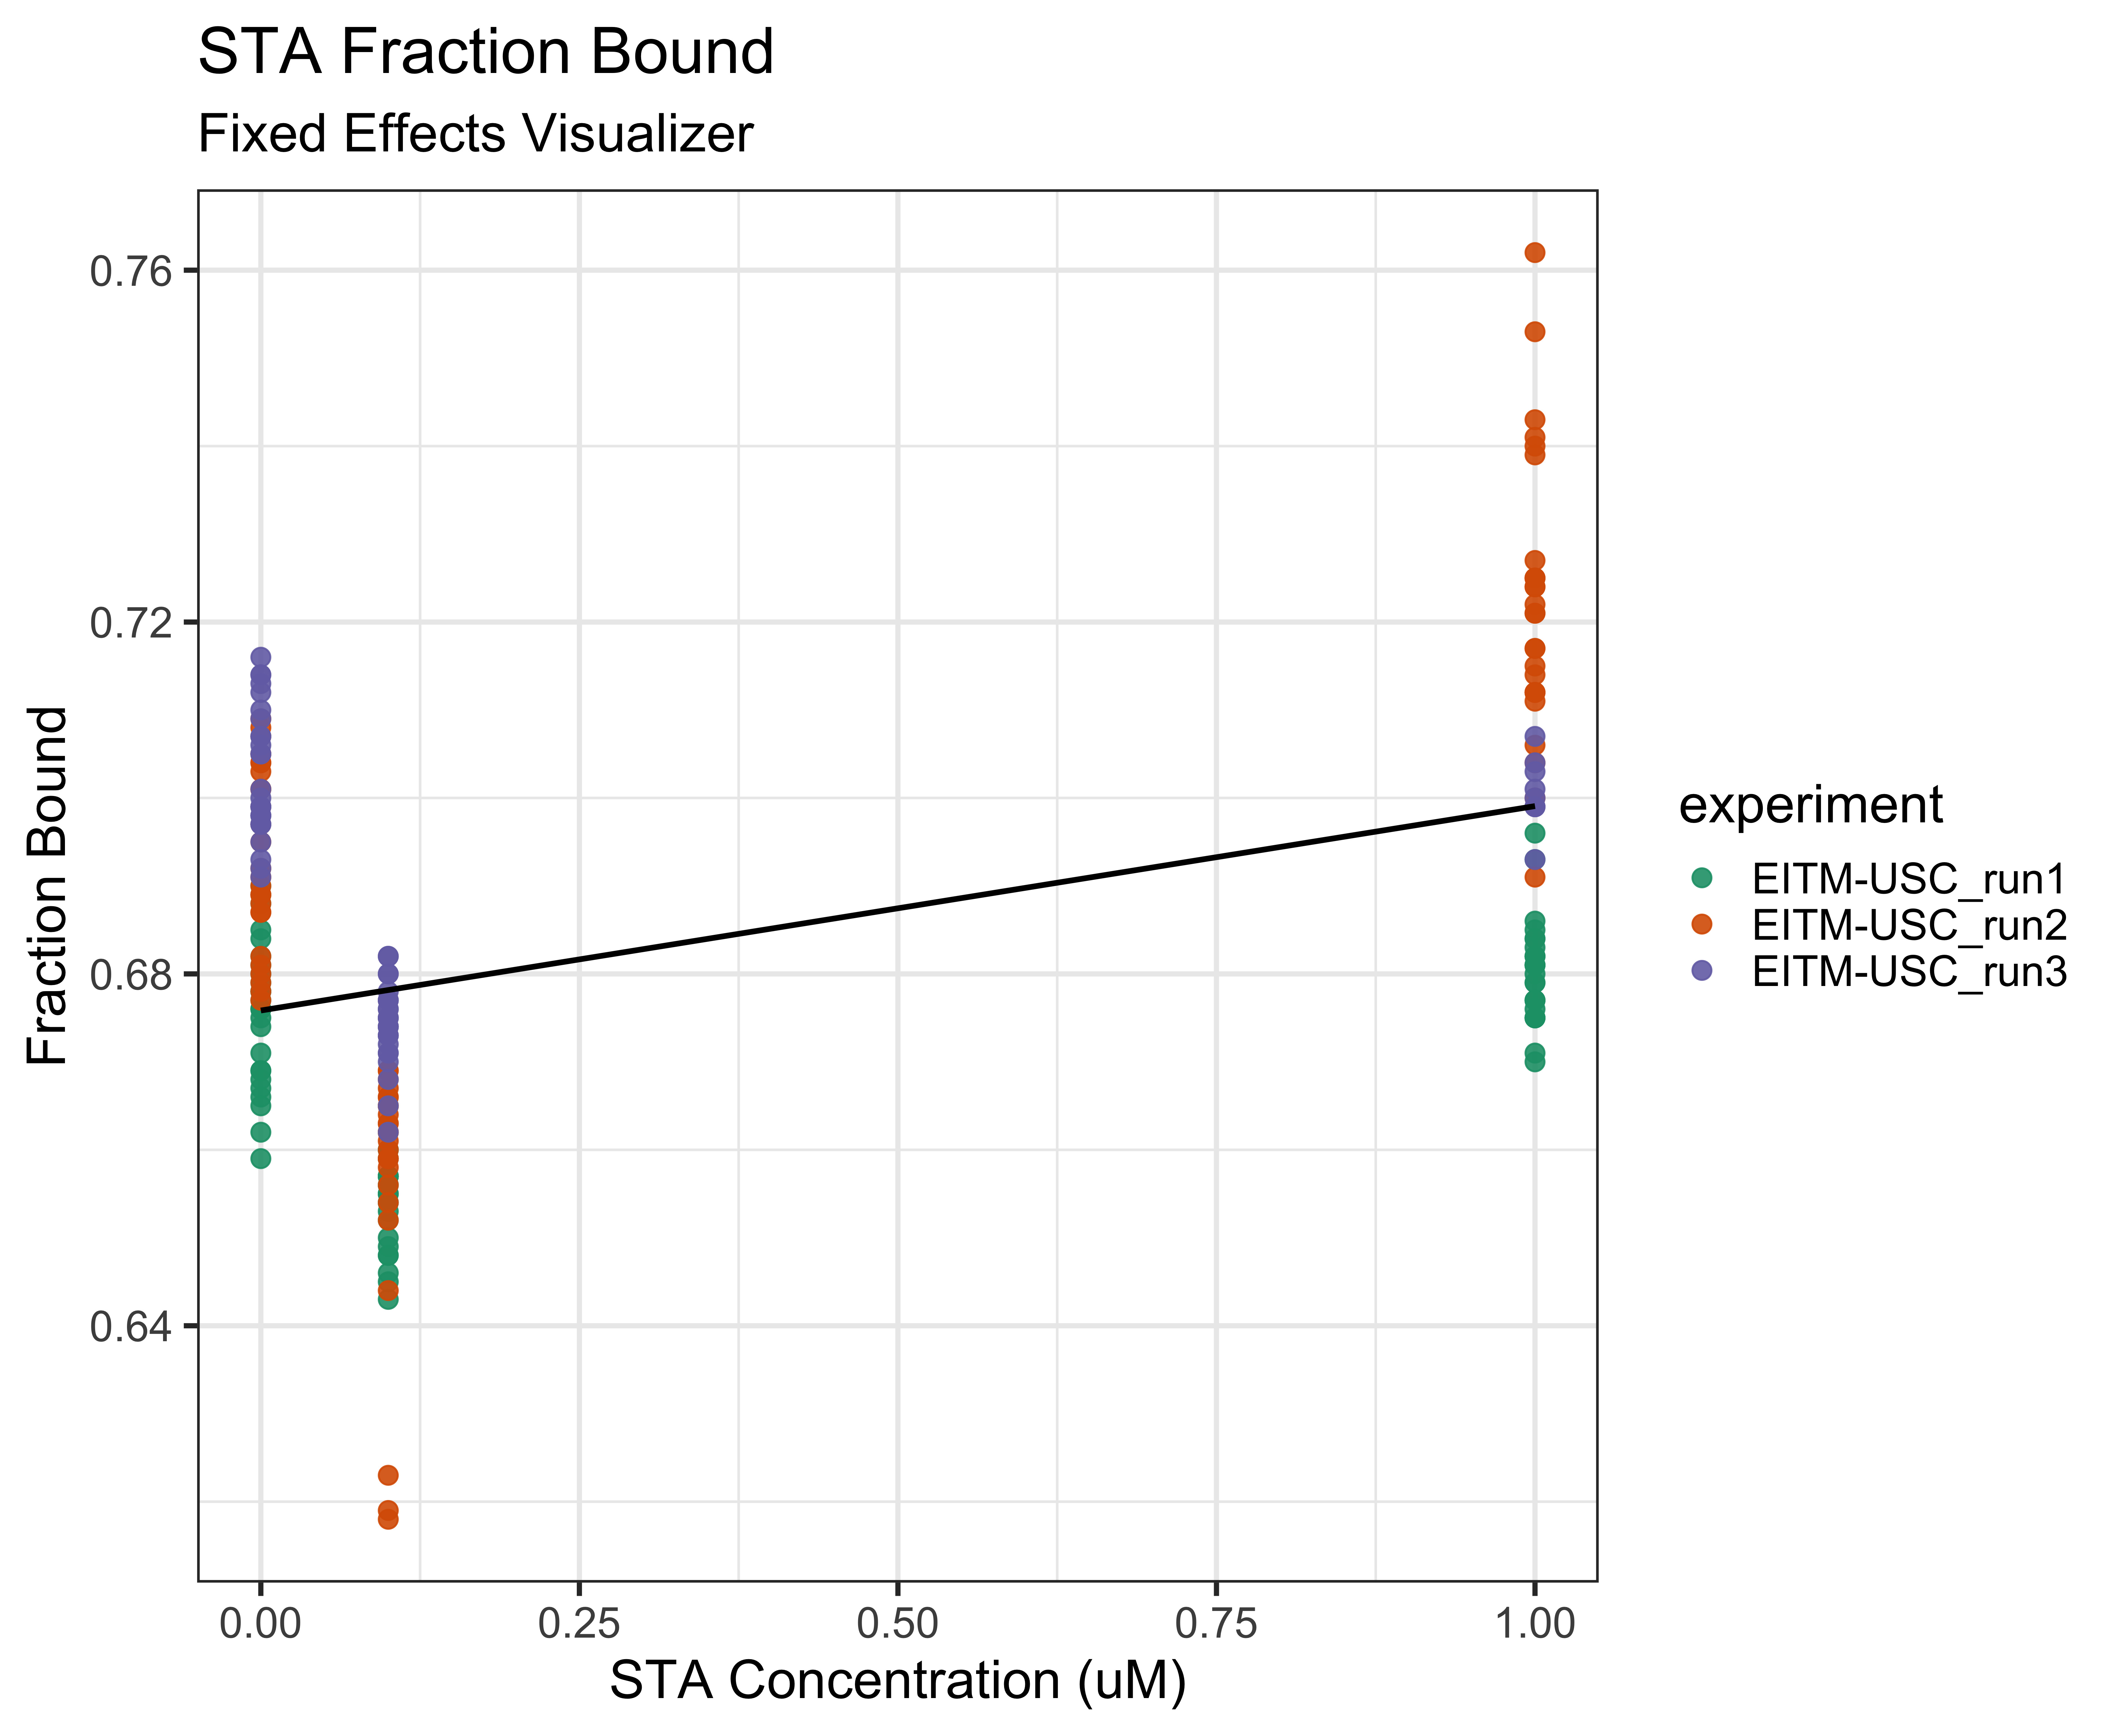
\includegraphics{FLIM_Analysis_Newdata_files/figure-latex/fixed-1.pdf}

This is a fixed linear model that only considers concentration and not
experiment in the model. Just looking at concentration, we observe that
fB slightly decreases as STA concentration increases.

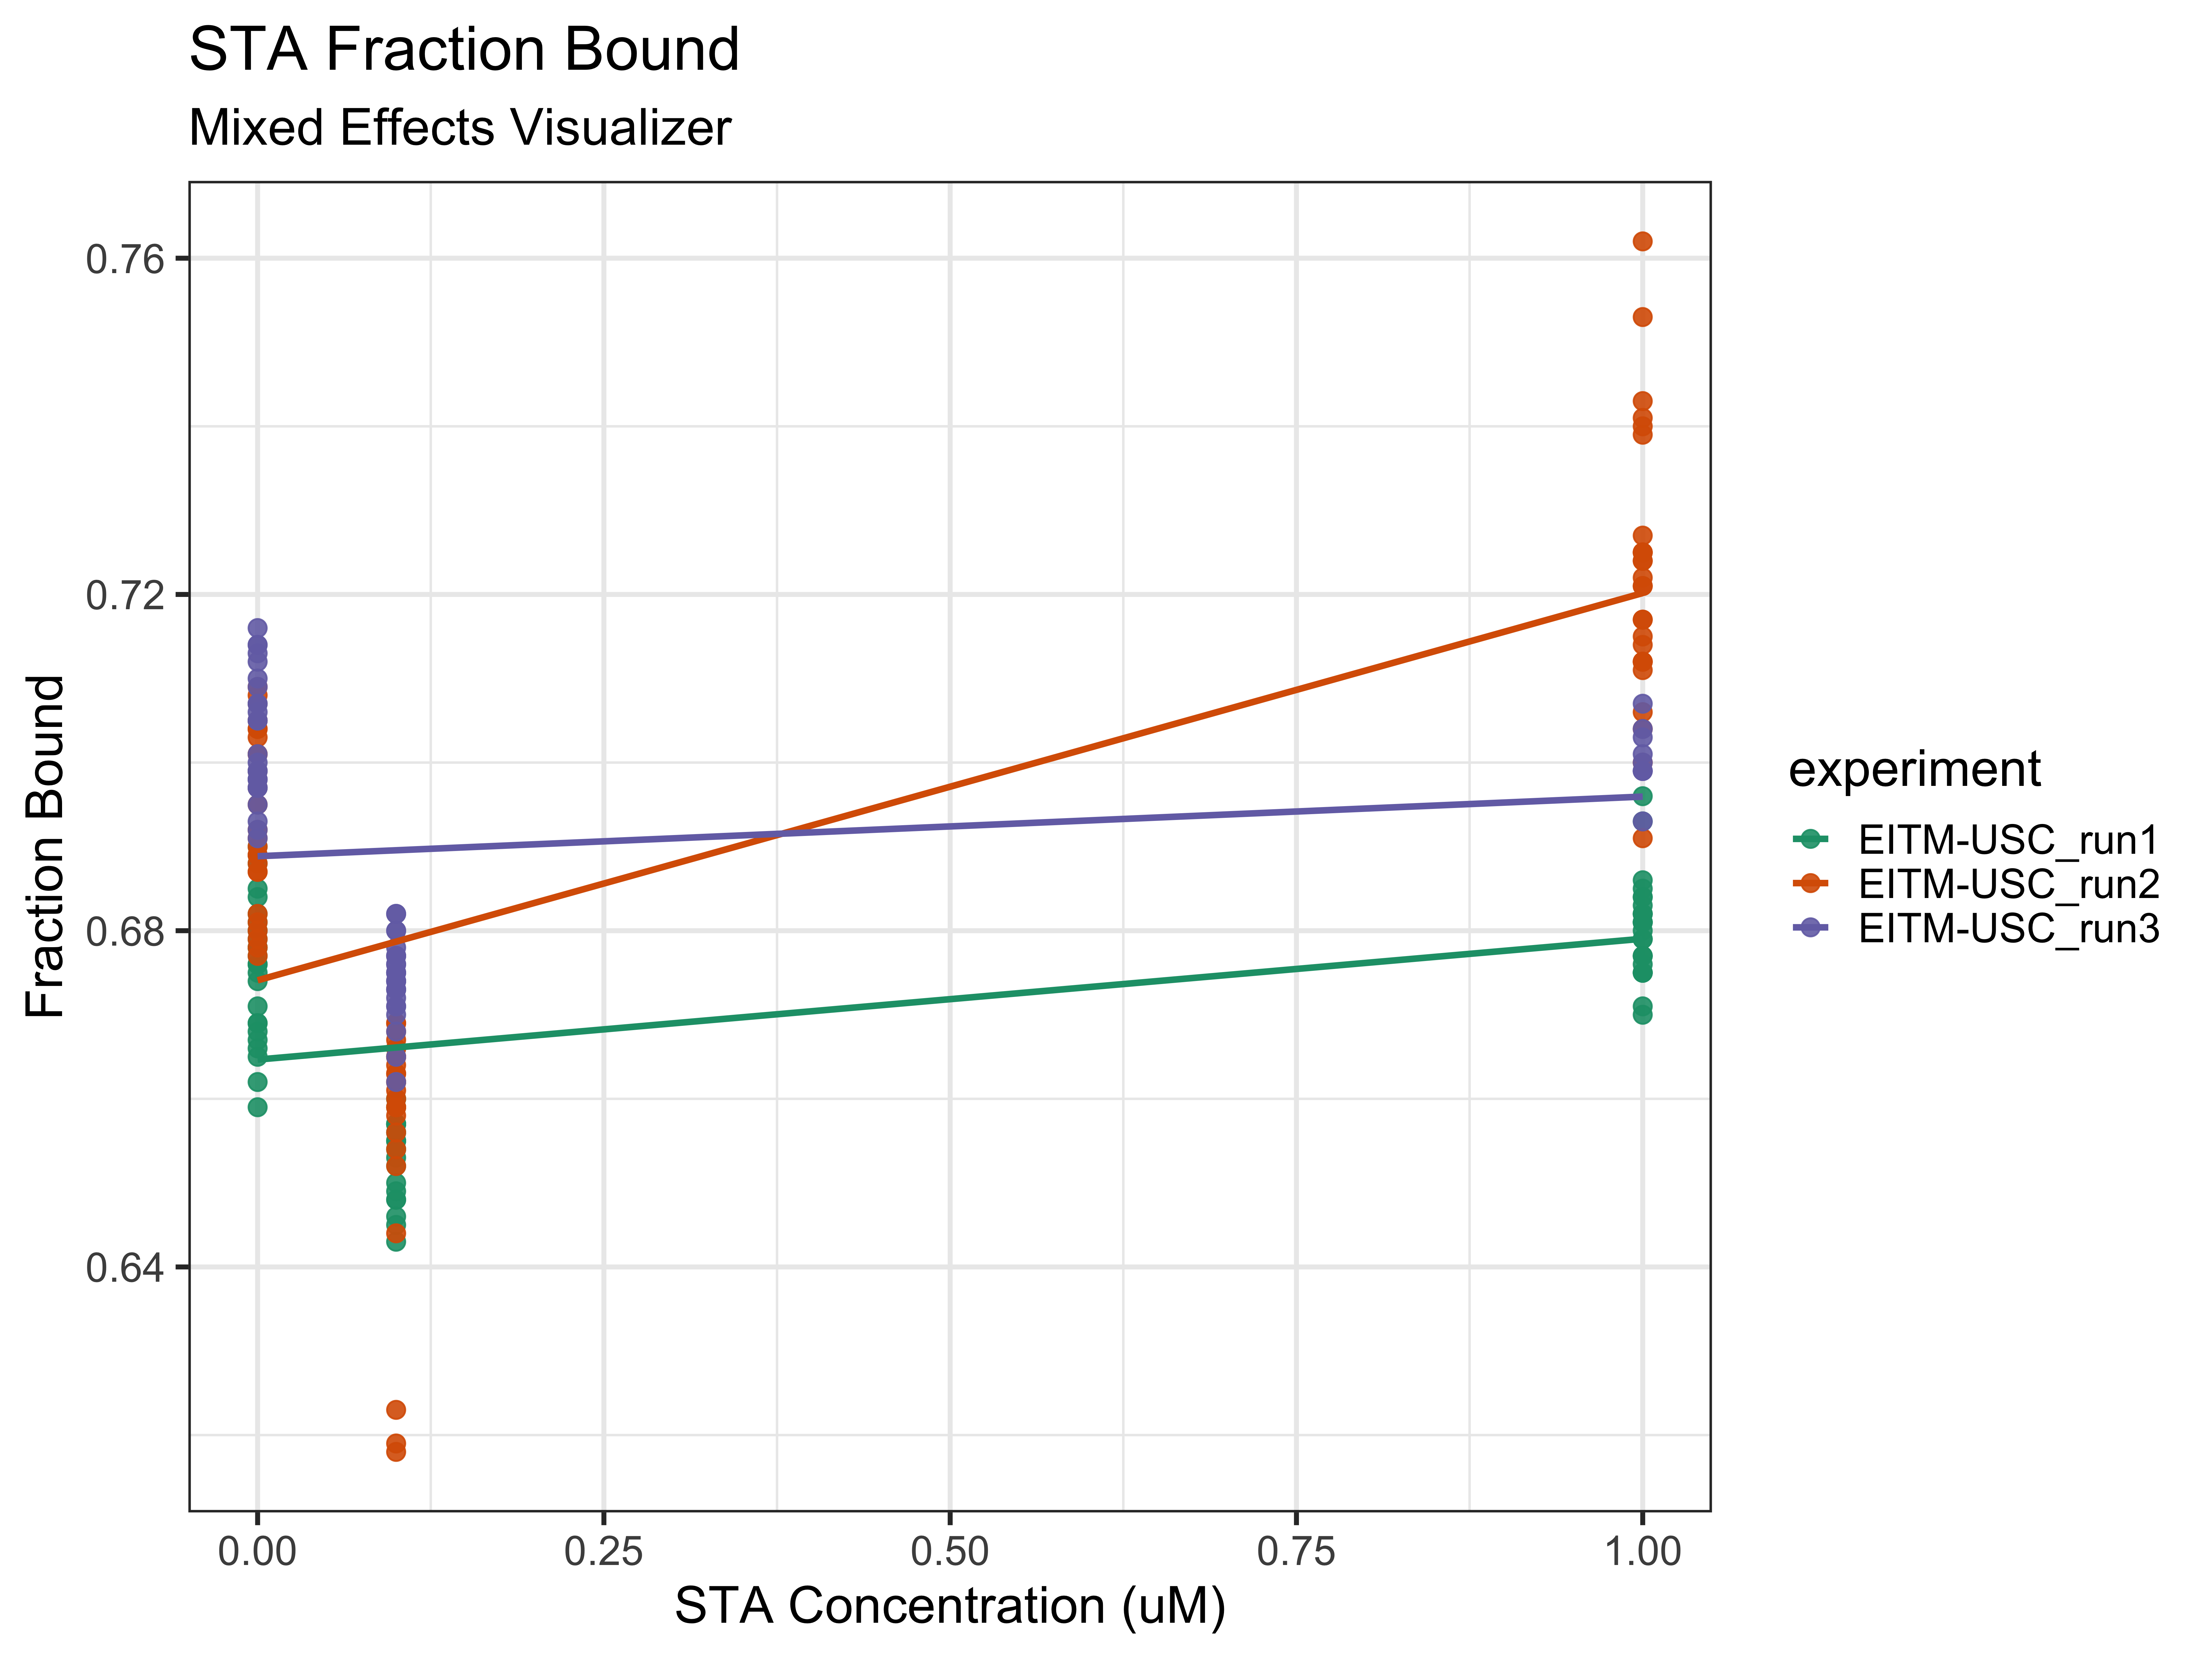
\includegraphics{FLIM_Analysis_Newdata_files/figure-latex/mem-1.pdf}

The mixed effect model shows us that the overall results are being
skewed by outliers from run 2. While run 1 and run 3 show a consistent
trend in how fraction bound responds to STA concentration, increasing fB
as concentration increases, run 2 deviates from that pattern and
decreases fB as concentration increases. This skews the results we see
in the fixed effects model. By including experiment as a random effect,
the model helps correct for the variability across runs and displays the
true relationship between STA and fB.

\begin{verbatim}
##                     Predictors     Estimates           CI      p
## 1                  (Intercept)          0.68  0.66 – 0.69 <0.001
## 2                Concentration         -0.00 -0.01 – 0.01  0.981
## 3               Random Effects                                  
## 4                           σ2          0.00                    
## 5                τ00Experiment          0.00                    
## 6                          ICC          0.34                    
## 7                 N Experiment             3                    
## 8                 Observations           225                    
## 9 Marginal R2 / Conditional R2 0.000 / 0.336
\end{verbatim}

\end{document}
